Python se destaca por su legibilidad y simplicidad. Algunas pautas importantes de la sintaxis incluyen:

\subsection{Variables y asignaciones}
Las variables en Python son contenedores que se utilizan para almacenar datos. Estos datos pueden ser números, cadenas de texto, listas, objetos o cualquier otro tipo de información que necesites en tu programa. Las variables te permiten acceder, modificar y manipular datos de manera dinámica en tu código.\\

Declaración y Asignación: Para crear una variable en Python, simplemente elige un nombre descriptivo y utiliza el operador de asignación ``$=$'' para darle un valor. La estructura general es la siguiente:

\begin{figure}[h]
    \centering
    \scalebox{0.35}{
    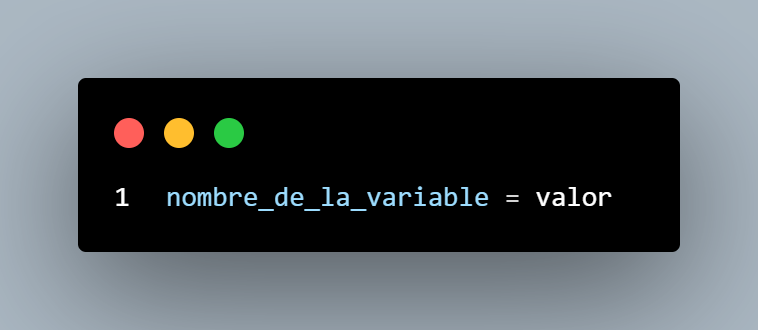
\includegraphics{Imagenes/funadamentos1.png}
    }
  \end{figure}

\begin{itemize}
    \item ``nombre\_de\_la\_variable'': Es el nombre que eliges para la variable. Debe seguir las reglas de nomenclatura y convenciones de nombres que se mencionaron previamente.  
    \item ``valor'': Es el dato que deseas almacenar en la variable. Puede ser un número, una cadena de texto, un resultado de cálculos, una lista, un objeto, etc.
\end{itemize}

\begin{figure}[h]
    \centering
    \scalebox{0.35}{
    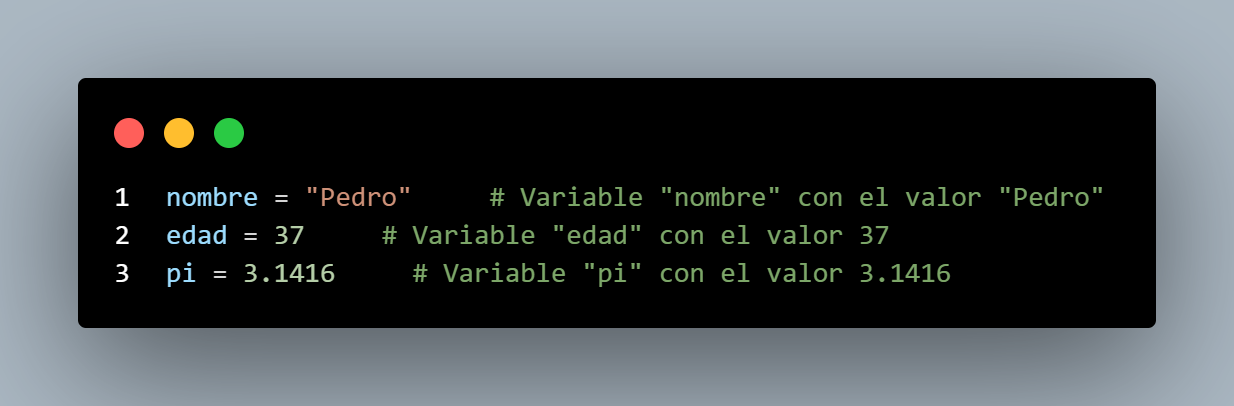
\includegraphics{Imagenes/fundamentos2.png}
    }
  \end{figure}

Reasignación de variables: Puedes cambiar el valor de una variable en cualquier momento asignándole un nuevo valor:\\
\begin{figure}[h]
    \centering
    \scalebox{0.35}{
    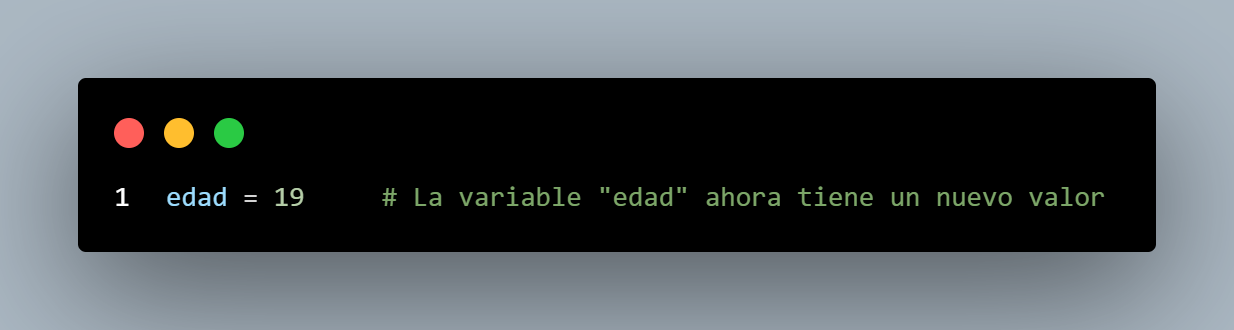
\includegraphics{Imagenes/fundamentos3.png}
    }
  \end{figure}

Identificadores: Los identificadores son nombres que se utilizan para representar variables, funciones, clases y otros elementos en Python. Algunas reglas claves para los identificadores en Python son:

\begin{itemize}
    \item Deben comenzar con una letra (mayúscula o minúscula) o un guión bajo ``\_''.
    \item Pueden contener letras, números y guiones bajos.
    \item Python distingue entre mayúsculas y minúsculas, por lo que mi\_variable y Mi\_Variable son consideradas diferentes.
    \item No se pueden utilizar palabras clave de Python como identificadores. Las palabras clave son términos reservados para funciones y estructuras de control, como ``if'', ``for'', ``while'', entre otros.
\end{itemize}

\begin{figure}[h]
    \centering
    \scalebox{0.35}{
    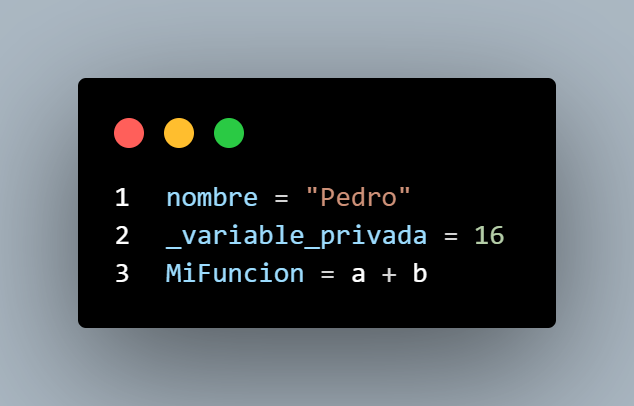
\includegraphics{Imagenes/fundamentos4.png}
    }
  \end{figure}

Uso de variables: Las variables se utilizan para almacenar valores y realizar cálculos. Puedes utilizar variables en expresiones matemáticas, en operaciones de cadena de texto, en estructuras de control (como condicionales y bucles) y para muchas otras tareas en tu programa.\\

\begin{figure}[h]
    \centering
    \scalebox{0.35}{
    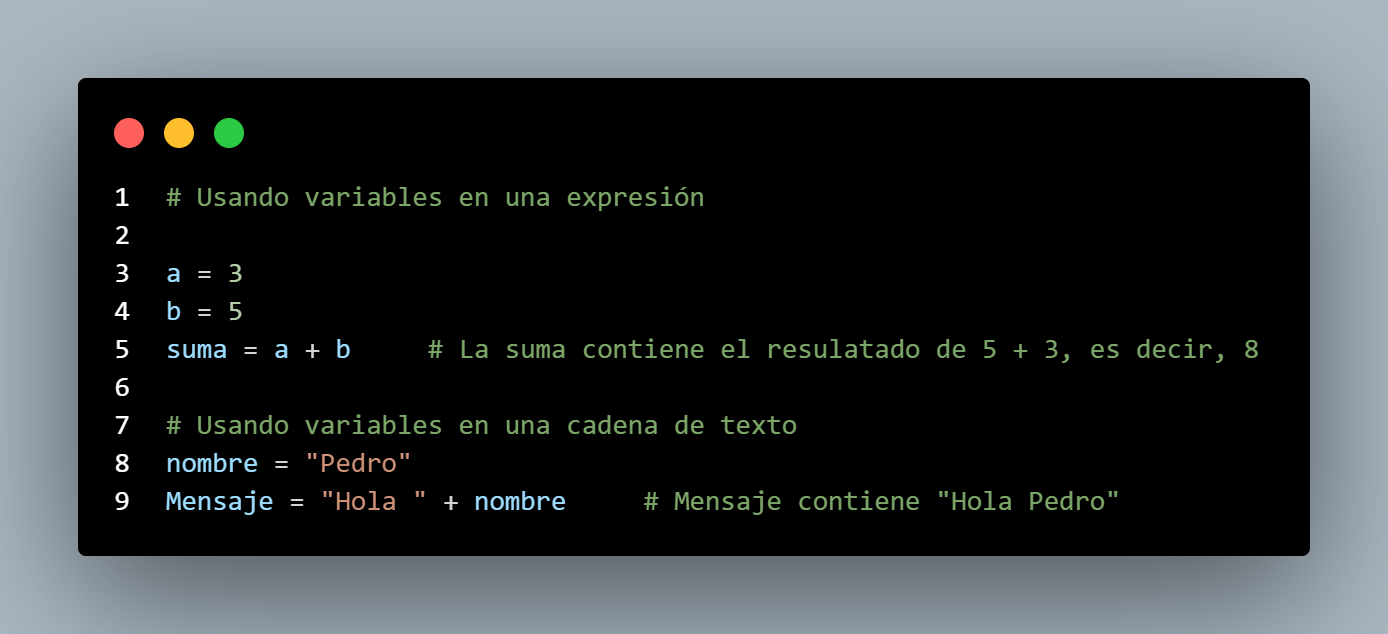
\includegraphics{Imagenes/fundamentos5.png}
    }
  \end{figure}

Constantes: Puedes usar variables para definir constantes, que son valores que no deben modificarse a lo largo del programa. Para indicar que una variable es una constante, es común utilizar letras mayúsculas y subrayados (por ejemplo, PI = 3.1416).\\

Desestructuración de Asignación: Python permite asignar valores a Múltiples variables en una sola línea de código. Esto es especialmente útil cuando se trabaja con secuencias como listas o tuplas.

\begin{figure}[h]
    \centering
    \scalebox{0.35}{
    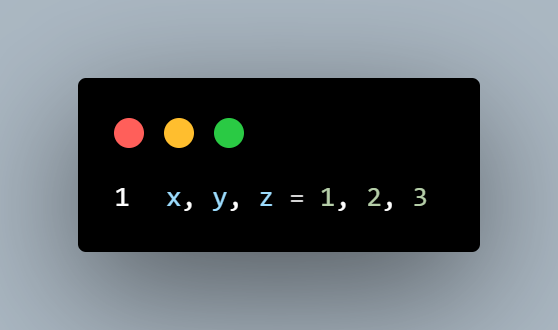
\includegraphics{Imagenes/fundamentos6.png}
    }
  \end{figure}

Operadores de Asignación Combinada: Python ofrece operadores de asignación combinada que permiten simplificar la asignación de variables en operaciones comunes. Por ejemplo, ``+='' es una forma abreviada de incrementar el valor de una variable.\\

\begin{figure}[h]
    \centering
    \scalebox{0.35}{
    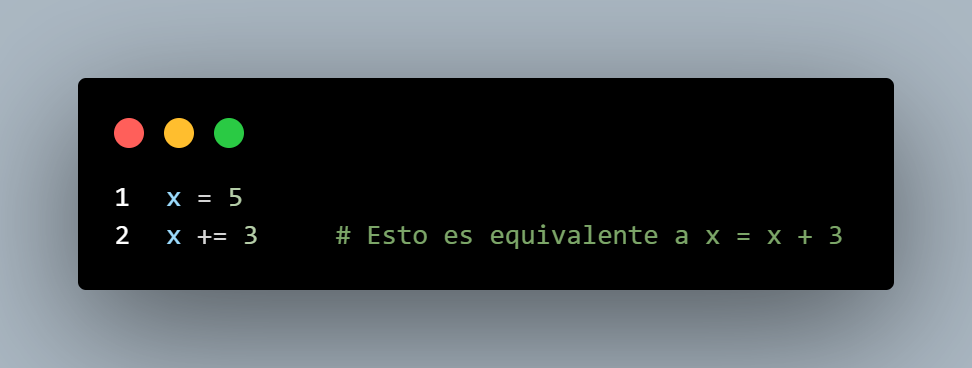
\includegraphics{Imagenes/fundamentos7.png}
    }
  \end{figure}

Tipos de datos: Python es un lenguaje de tipo dinámico, lo que significa que una variable no tiene un tipo de dato fijo. El tipo de dato de una variable se asigna automáticamente según el valor que contiene. Puedes verificar el tipo de dato de una variable utilizando la función ``type()'':\\

\begin{figure}[h]
    \centering
    \scalebox{0.35}{
    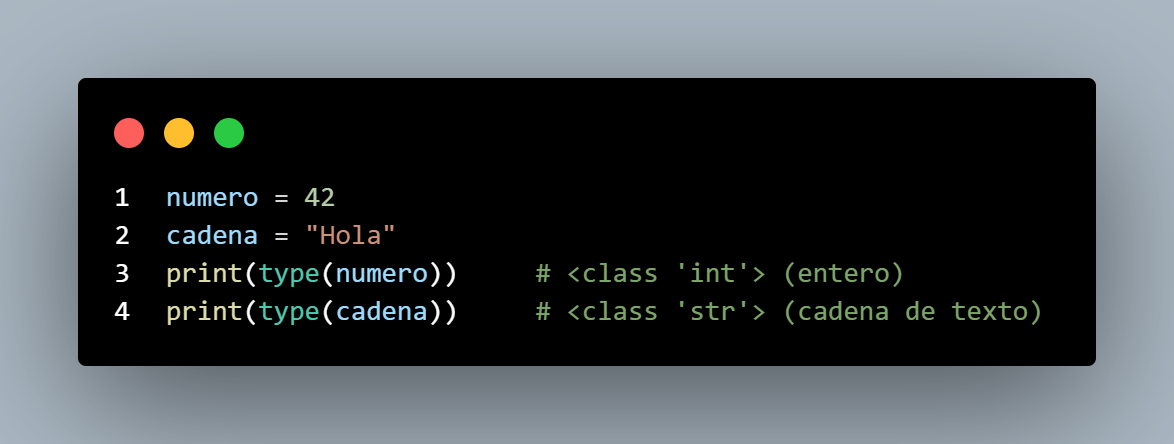
\includegraphics{Imagenes/fundamentos8.png}
    }
  \end{figure}

Ámbito de variables: Las variables pueden tener un ámbito local o global:
\begin{itemize}
    \item Ámbito local: Las variables declaradas dentro de una función tienen un ámbito local y solo son accesibles dentro de esa función.
    \begin{figure}[h]
        \centering
        \scalebox{0.35}{
        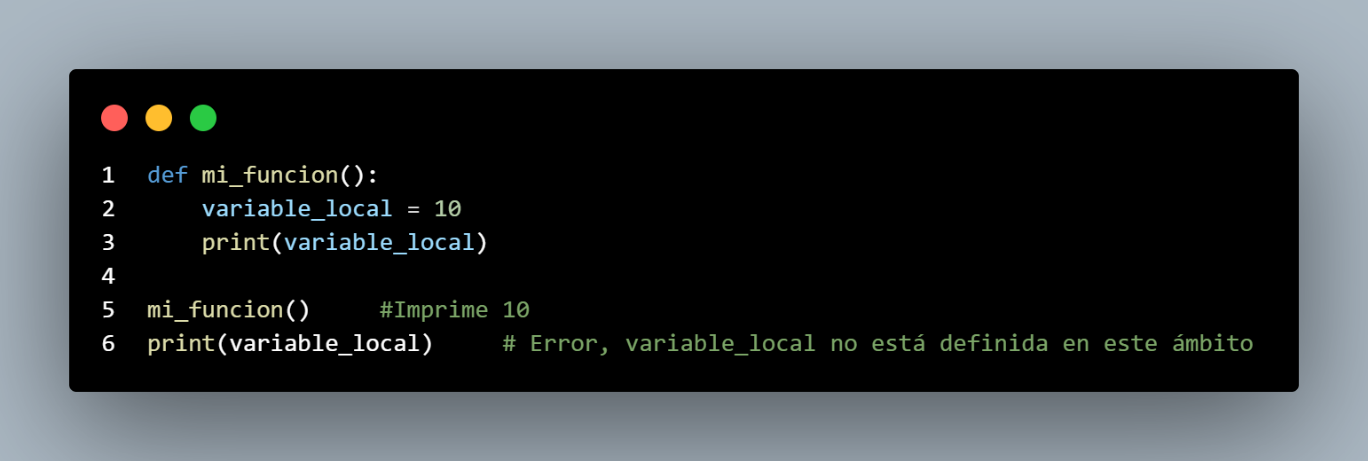
\includegraphics{Imagenes/fundamentos9.png}
        }
      \end{figure}
    \item Ámbito Global: Las variables declaradas fuera de una función o declaradas como globales dentro de una función tienen un ámbito global y son accesibles desde cualquier parte del código.
    \begin{figure}[h]
        \centering
        \scalebox{0.35}{
        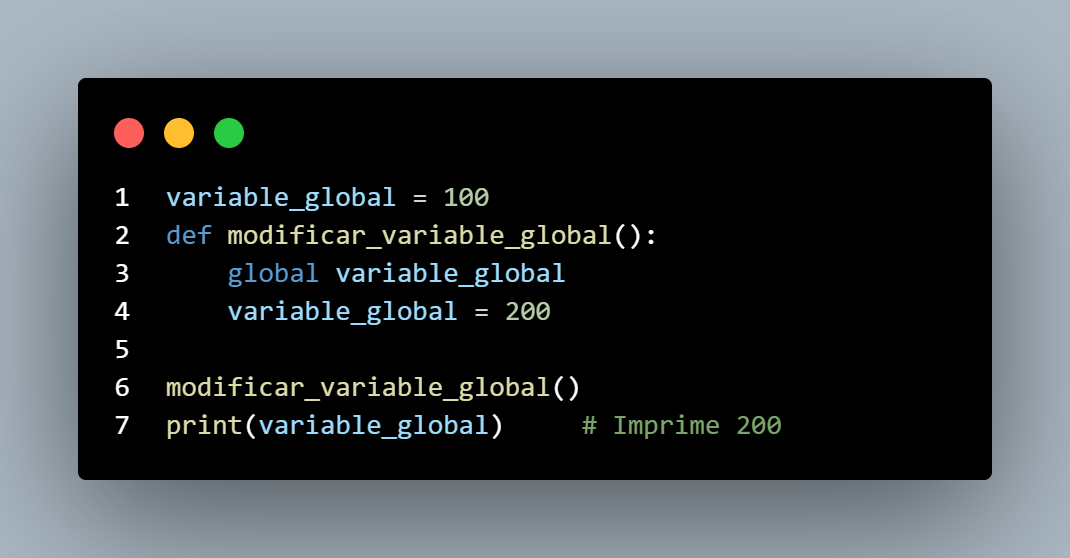
\includegraphics{Imagenes/fundamentos10.png}
        }
      \end{figure}
\end{itemize}
Ejemplo usando ambos:

\begin{figure}[h]
    \centering
    \scalebox{0.35}{
    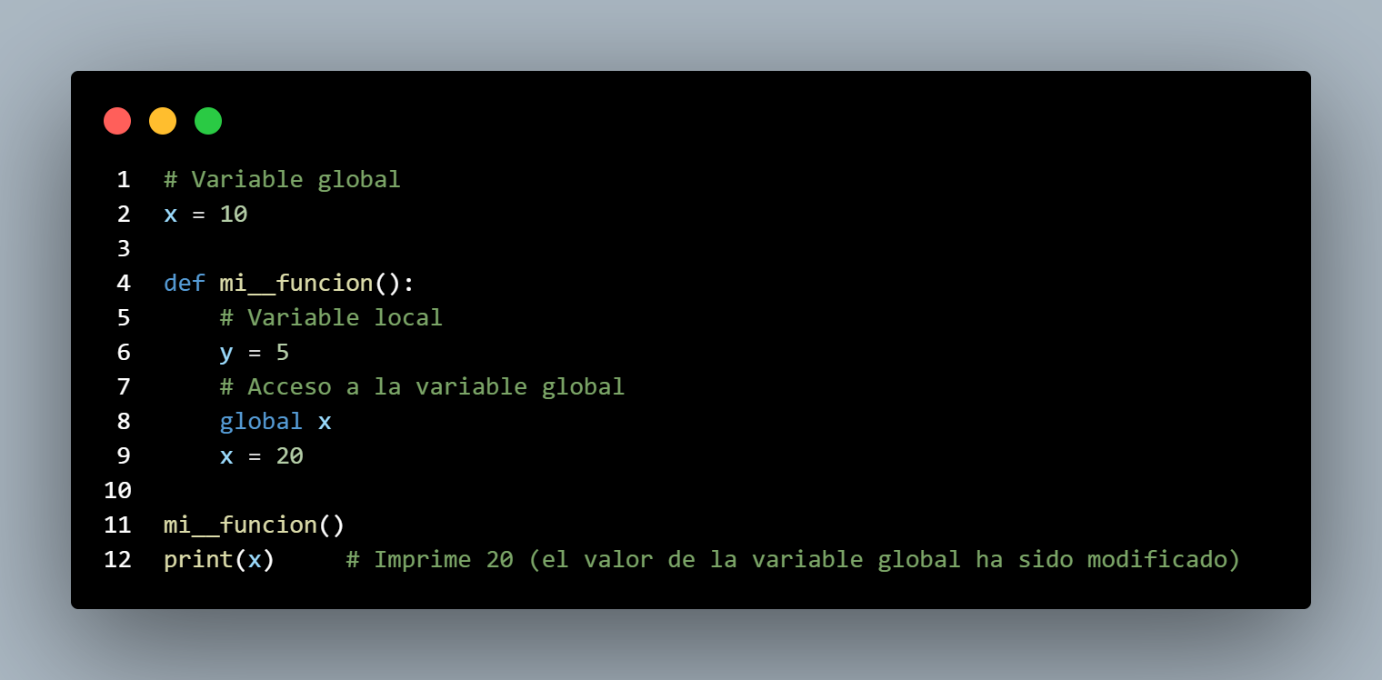
\includegraphics{Imagenes/fundamentos11.png}
    }
  \end{figure}

Estos son algunos aspectos adicionales relacionados con las variables en Python que pueden ser útiles para comprender en tu proceso de aprendizaje.

\subsection{Operadores Aritmeticos}
Los operadores aritméticos en Python se utilizan para realizar operaciones matemáticas. 

Los principales son:
\begin{itemize}
    \item Suma (+): Se utiliza para sumar dos valores.
    \item Resta (-): Se utiliza para restar un valor de otro.
    \item Multiplicación (*): Se utiliza para multiplicar dos valores.
    \item División (/): Se utiliza para dividir un valor por otro.
    \item División Entera (//): Devuelve la parte entera de la división entre dos valores.
    \item Módulo (\%): Devuelve el resto de la división entre dos valores.
    \item Potencia (**): Eleva un valor a una potencia.
  \end{itemize}  

\subsection{Operadores de comparación}
Los operadores de comparación se utilizan para comparar dos valores y devuelven un valor booleano (True o False). 

Los principales son:
\begin{itemize}
    \item Igual (==): Comprueba si dos valores son iguales.
    \item No Igual (!=): Comprueba si dos valores no son iguales.
    \item Mayor que (>): Comprueba si un valor es mayor que otro. En caso de strings se compara cadenas de caracteres lexicográficamente (es decir, en función del orden alfabético).
    \item Menor que (<): Comprueba si un valor es menor que otro.En caso de strings se compara cadenas de caracteres lexicográficamente (es decir, en función del orden alfabético).
    \item Mayor o igual que (>=): Comprueba si un valor es mayor o igual que otro.En caso de strings se compara cadenas de caracteres lexicográficamente (es decir, en función del orden alfabético).
    \item Menor o igual que (<=): Comprueba si un valor es menor o igual que otro. En caso de strings se compara cadenas de caracteres lexicográficamente (es decir, en función del orden alfabético).
\end{itemize}

\subsection{Operadores lógicos}
Los operadores lógicos se utilizan para combinar expresiones lógicas y devuelven un valor booleano. 

Los principales son:
\begin{itemize}
    \item and: Devuelve True si ambas expresiones son True.
    \item or: Devuelve True si al menos una de las expresiones es True.
    \item not: Devuelve el inverso de la expresión.
\end{itemize}

\subsection{Operadores de asignación}
Los operadores de asignación se utilizan para asignar valores a variables. Algunos de ellos incluyen:
\begin{itemize}
    \item =: Asigna un valor a una variable.
    \item +=: Suma y asigna el resultado a la variable.
    \item -=: Resta y asigna el resultado a la variable.
    \item *=: Multiplica y asigna el resultado a la variable.
    \item /=: Divide y asigna el resultado a la variable.
\end{itemize}

\subsection{Operadores de pertenencia e identidad}
\begin{itemize}
    \item Operadores de Pertenencia: `in` y `not in` se utilizan para verificar si un elemento está presente en una secuencia (como una lista, tupla, etc.)
    \item Operadores de Identidad: `is` y `is not` se utilizan para verificar si dos objetos tienen la misma identidad (es decir, si son el mismo objeto en la memoria).
\end{itemize}

\subsection{Expresiones}
Una expresión es una combinación de valores, variables y operadores que se evalúa para producir un resultado. Las expresiones se utilizan en muchas partes del código, como asignaciones, condicionales, bucles y funciones. Por ejemplo:\\

\begin{figure}[h]
    \centering
    \scalebox{0.35}{
    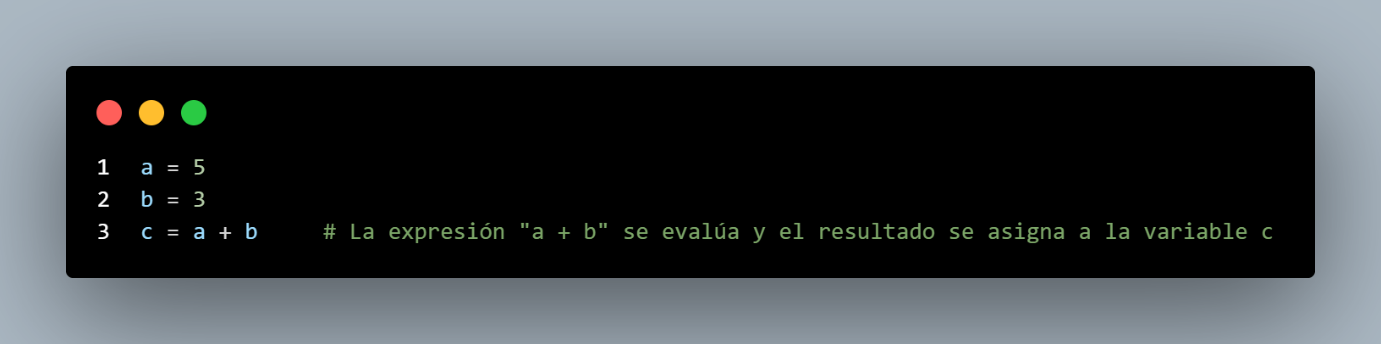
\includegraphics{Imagenes/fundamentos12.png}
    }
  \end{figure}
Las expresiones pueden ser tan simples como una sola variable o tan complejas como cálculos matemáticos o lógicos.

Estos son los operadores y las expresiones en Python que son fundamentales para realizar tareas de cálculo, toma de decisiones y procesamiento de datos en tus programas. Puedes combinar estos operadores y expresiones de diversas maneras para realizar tareas específicas en tu código.

\subsection{Comentarios y formato de código}
Los comentarios y el formato de código son aspectos cruciales de la programación en Python. Los comentarios son notas en el código que se utilizan para explicar lo que hace el código, mientras que el formato se refiere a la estructura y el estilo del código para que sea más legible y mantenible.\\

Comentarios: Los comentarios en Python se utilizan para agregar explicaciones o notas al código fuente. Se inician con el símbolo ``\#'' y Python los ignoran durante la ejecución. Los comentarios son útiles para documentar el código y facilitar su comprensión tanto para el programador como para otros colaboradores. 
\begin{figure}[h]
    \centering
    \scalebox{0.35}{
    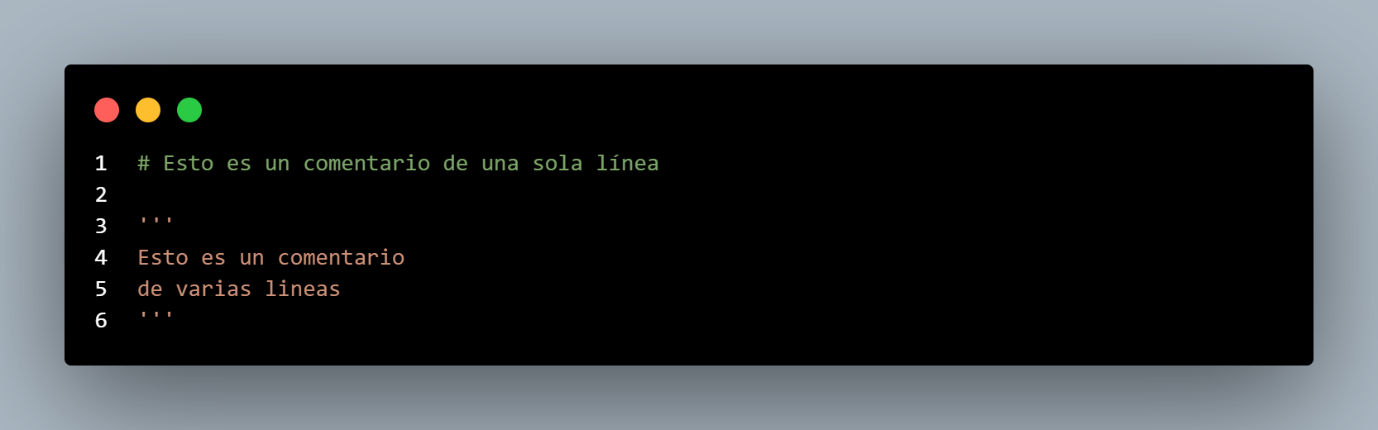
\includegraphics{Imagenes/fundamentos13.png}
    }
  \end{figure}
\begin{itemize}
    \item Comentarios de una sola línea: Se utilizan para incluir explicaciones breves en una línea.
    \item Comentarios de varias líneas: Se utilizan para describir secciones de código más largas y pueden abarcar varias líneas.
\end{itemize}

Formato de Código: El formato del código es importante para mantener la legibilidad y la consistencia en un proyecto. Python se destaca por su énfasis en la indentación (espacios al principio de una línea) para delimitar bloques de código. 
\begin{itemize}
    \item Indentación: La sangría en Python es fundamental para definir bloques de código. A diferencia de otros lenguajes que utilizan llaves o paréntesis para delimitar bloques, en Python, la sangría se utiliza para indicar la estructura del programa. Esto fomenta la legibilidad y la claridad del código. Un bloque de código se define mediante el uso de espacios o tabulaciones con un mismo nivel de sangría. 
\begin{figure}[h]
    \centering
    \scalebox{0.35}{
    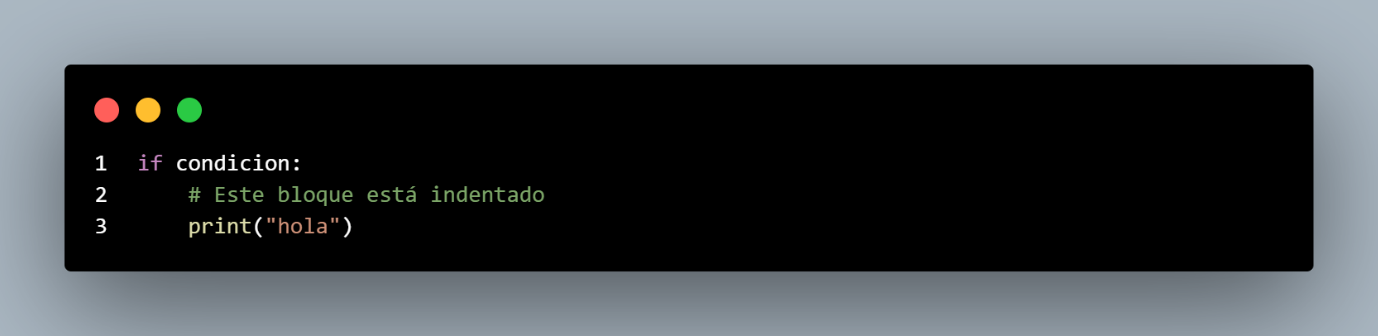
\includegraphics{Imagenes/fundamentos14.png}
    }
    \end{figure}
    \item Interpretado: Python es un lenguaje de programación interpretado. Esto significa que no es necesario compilar el código fuente en código de máquina antes de ejecutarlo. En cambio, el intérprete de Python lee y ejecuta el código línea por línea en tiempo real. Esto facilita la depuración y la portabilidad, ya que un programa escrito en Python se puede ejecutar en cualquier sistema que tenga un intérprete de Python instalado.
\begin{figure}[h]
    \centering
    \scalebox{0.35}{
    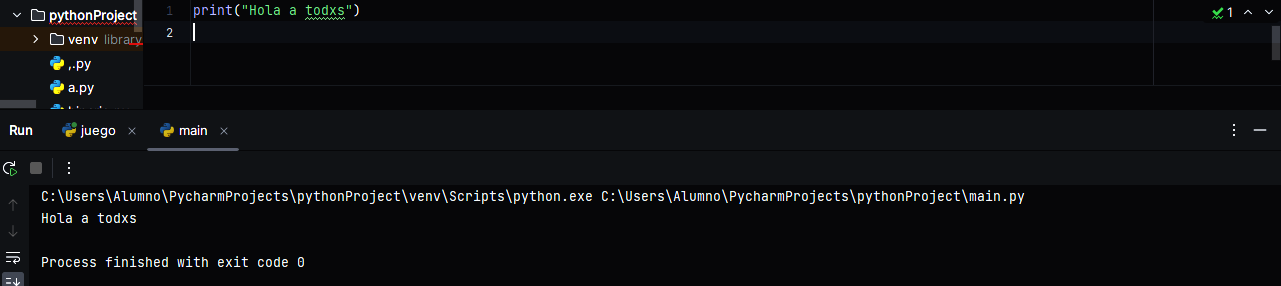
\includegraphics{Imagenes/fundamentos15.png}
    }
    \end{figure}
    \item Tipado dinámico: Python es un lenguaje de tipado dinámico, lo que significa que no necesitas declarar explícitamente el tipo de una variable al crearla. El tipo de una variable se determina automáticamente en el tiempo de ejecución según el valor que contiene. Esto permite una mayor flexibilidad, pero también significa que debes tener cuidado con los tipos de datos para evitar errores inesperados. 
\begin{figure}[h]
    \centering
    \scalebox{0.35}{
    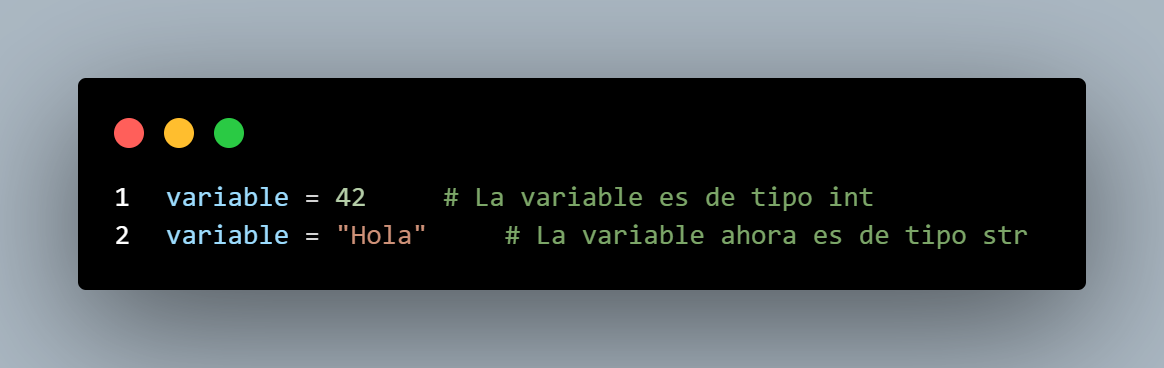
\includegraphics{Imagenes/fundamentos16.png}
    }
    \end{figure}
    \item Convenciones de Nombres: En Python, se siguen ciertas convenciones para nombrar variables, funciones y clases. Algunas pautas comunes incluyen:

\begin{itemize}
    \item Los operadores y las expresiones son componentes esenciales en Python y en la programación en general. Los operadores se utilizan para realizar operaciones en variables y valores, mientras que las expresiones son combinaciones de variables, valores y operadores que se evalúan para producir un resultado. 
    \item Variables y funciones: Usar letras minúsculas y guiones bajos para separar palabras (ejemplo: mi\_variable, mi\_funcion).
    \item Clases: Usar CamelCase (iniciar cada palabra con mayúscula, sin espacios ni guiones bajos) (ejemplo: MiClase).
    \item Constantes:Los nombres de las constantes deben estar en mayúsculas. Si es necesario separar palabras en el nombre de la constante, se pueden usar guiones bajos. Por ejemplo, PI o TASA\_DE\_INTERES.
    \item Convenciones especificas: Para indicar que una variable o función es ``privada'' (es decir, no debería accederse desde fuera de su módulo), se puede anteponer un guion bajo al nombre, por ejemplo, \_variable\_privada. Para variables que actúan como constantes y no deberían modificarse, se puede utilizar un guion bajo en mayúsculas al principio del nombre, como \_CONSTANTE.
    \item Variables temporales: En bucles y expresiones cortas, es común usar nombres de variables temporales cortos como i, j, k para iteradores. Sin embargo, es importante que estos nombres sean descriptivos dentro del contexto.
\end{itemize}

    \item Espaciado: Agregar espacios alrededor de operadores y después de comas para mejorar la legibilidad.
    \begin{figure}[h]
        \centering
        \scalebox{0.35}{
        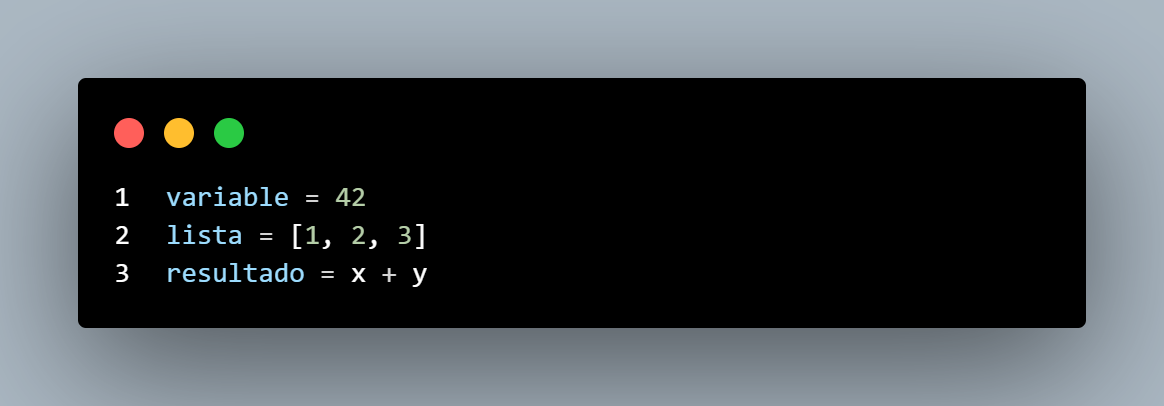
\includegraphics{Imagenes/fundamentos17.png}
        }
      \end{figure}
    \item Longitud de Línea: Es una buena práctica limitar la longitud de una línea de código a aproximadamente 79-80 caracteres para facilitar la lectura. Puedes usar una barra invertida \ para dividir una línea larga en varias líneas:
    \begin{figure}[h]
        \centering
        \scalebox{0.35}{
        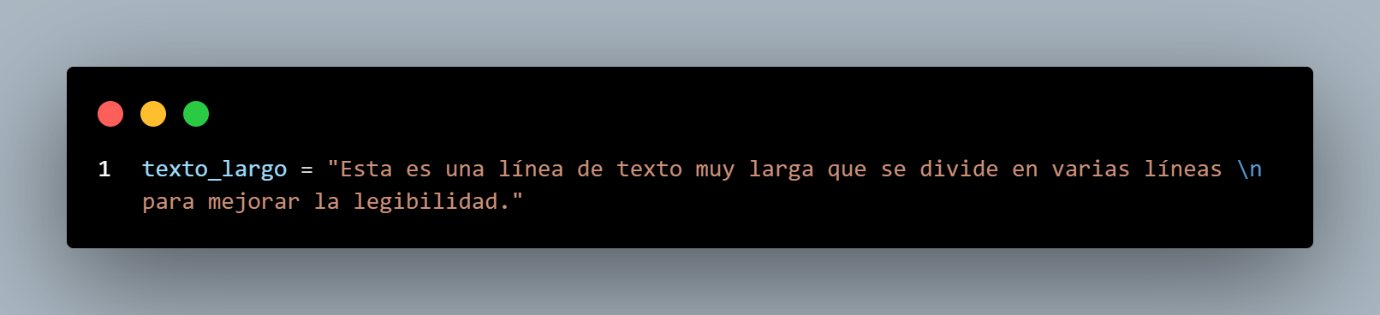
\includegraphics{Imagenes/fundamentos18.png}
        }
      \end{figure}
    \item Comentarios Descriptivos: Los comentarios deben ser informativos y explicar el propósito de una sección de código. Es especialmente útil para documentar partes complicadas o algoritmos. No es necesario comentar lo obvio.
\end{itemize}

El formato de código y los comentarios son esenciales para que tu código sea comprensible, colaborativo y mantenible. Adherirse a las convenciones de estilo y escribir comentarios informativos ayuda a otros programadores (y a ti mismo) a entender y mantener el código de manera más eficaz.
